\documentclass[a4paper,12pt,titlepage]{article}
\usepackage[utf8]{inputenc}
\usepackage{graphicx} % Required for inserting images
\usepackage[spanish,es-tabla]{babel}
\usepackage[none]{hyphenat}
\usepackage[justification=centering]{caption}
\usepackage{subcaption}
\usepackage{amssymb, amsmath}
\usepackage{gensymb}
\usepackage{fancyhdr}
\usepackage{wrapfig}
\usepackage{physics}
\usepackage[table,xcdraw]{xcolor}

\usepackage[a4paper]{geometry}
\geometry{top=3cm, bottom=3.0cm,left=2cm, right=2cm}


\lhead{Medida de la constante dieléctrica}
\rhead{Gonzalo Bastos González}

\pagestyle{fancy}

\title{Medida de la constante dieléctrica}
\author{Gonzalo Bastos González}
\date{Técnicas expermimentales II-Laboratorio de electromagnetismo}

\begin{document}

\maketitle
\tableofcontents

\newpage

\section{Objetivos e introducción teórica}

El objetivo de esta práctica es determinar la permitividad del vacío, $\epsilon_0$, estudiando la relación entre carga y voltaje de un condensador plano. Además de eso, determinaremos la permitividad de un dieléctrico con el mismo método.

Para todas estas medidas partiremos de un condensador plano-paralelo, que supondremos ideal, ya que su superficie es mucho mayor que la distancia a la que estarán separadas las placas en todo momento y, por tanto, podremos despreciar los efectos de borde. La capacidad de nuestro condensador plano-paralelo ideal en el vacío viene dada por la siguiente expresión:

\begin{equation}
    C =\frac{Q}{V} \Rightarrow C_0 = \frac{\epsilon_0S}{d}
    \label{C1}
\end{equation}

Donde S es la superficie de las placas y d la distancia entre ellas. En un medio dieléctrico la capacidad es:

\begin{equation}
    C = \frac{\epsilon_0 \epsilon_r S}{d}
    \label{C2}
\end{equation}

Donde $\epsilon_r$ es la permitividad relativa del dieléctrico. Cabe destacar también que durante toda nuestra práctica estamos trabajando con la aproximación de que estamos en el vacío, que es válida teniendo en cuenta que la permitividad relativa del aire tiene el siguiente valor:

\begin{equation}
    \epsilon_r = 1,0005364 \simeq 1
\end{equation}

De las ecuaciones (\ref{C1}) y (\ref{C2}) se deduce la siguiente relación para la permitividad relativa de nuestro dieléctrico:

\begin{equation}
    \epsilon_r = \frac{C}{C_0}
    \label{e_r}
\end{equation}

\section{Materiales y metodología}

Los materiales e instrumentos empleados durante la práctica fueron:

\begin{enumerate}
    \item Condensador plano-paralelo de radio $r=13 \;cm$. Este es el condensador que usaremos para medir, donde variaremos la distancia y introduciremos el dieléctrico.
    \item Condensador de medida, $C_M$. Lo emplearemos como referencia y tiene una capacidad conocida de $220 \;nF$, que es mucho mayor que la del condensador plano.
    \item Fuente de alimentación, proporciona una diferencia de potencial $V_0$ de entre 1 y 5 $kV$.
    \item Amplificador de señal. Se emplea con ganancia unidad, su función es permitir la medida del voltaje en el condensador de medida $C_M$ a través de una alta impedancia de entrada. De este modo evitamos la descarga de $C_M$ durante la medida.
    \item Polímetro que con el que mediremos la diferencia de potencial del condensador de medida.
    \item Resistencia de $10\; M\Omega$, que se conectará con la fuente en serie por motivos de seguridad.
    \item Cables de conexión.
\end{enumerate}

\begin{figure}[h!]
    \centering
    \begin{subfigure}{0.45\textwidth}
        \centering
        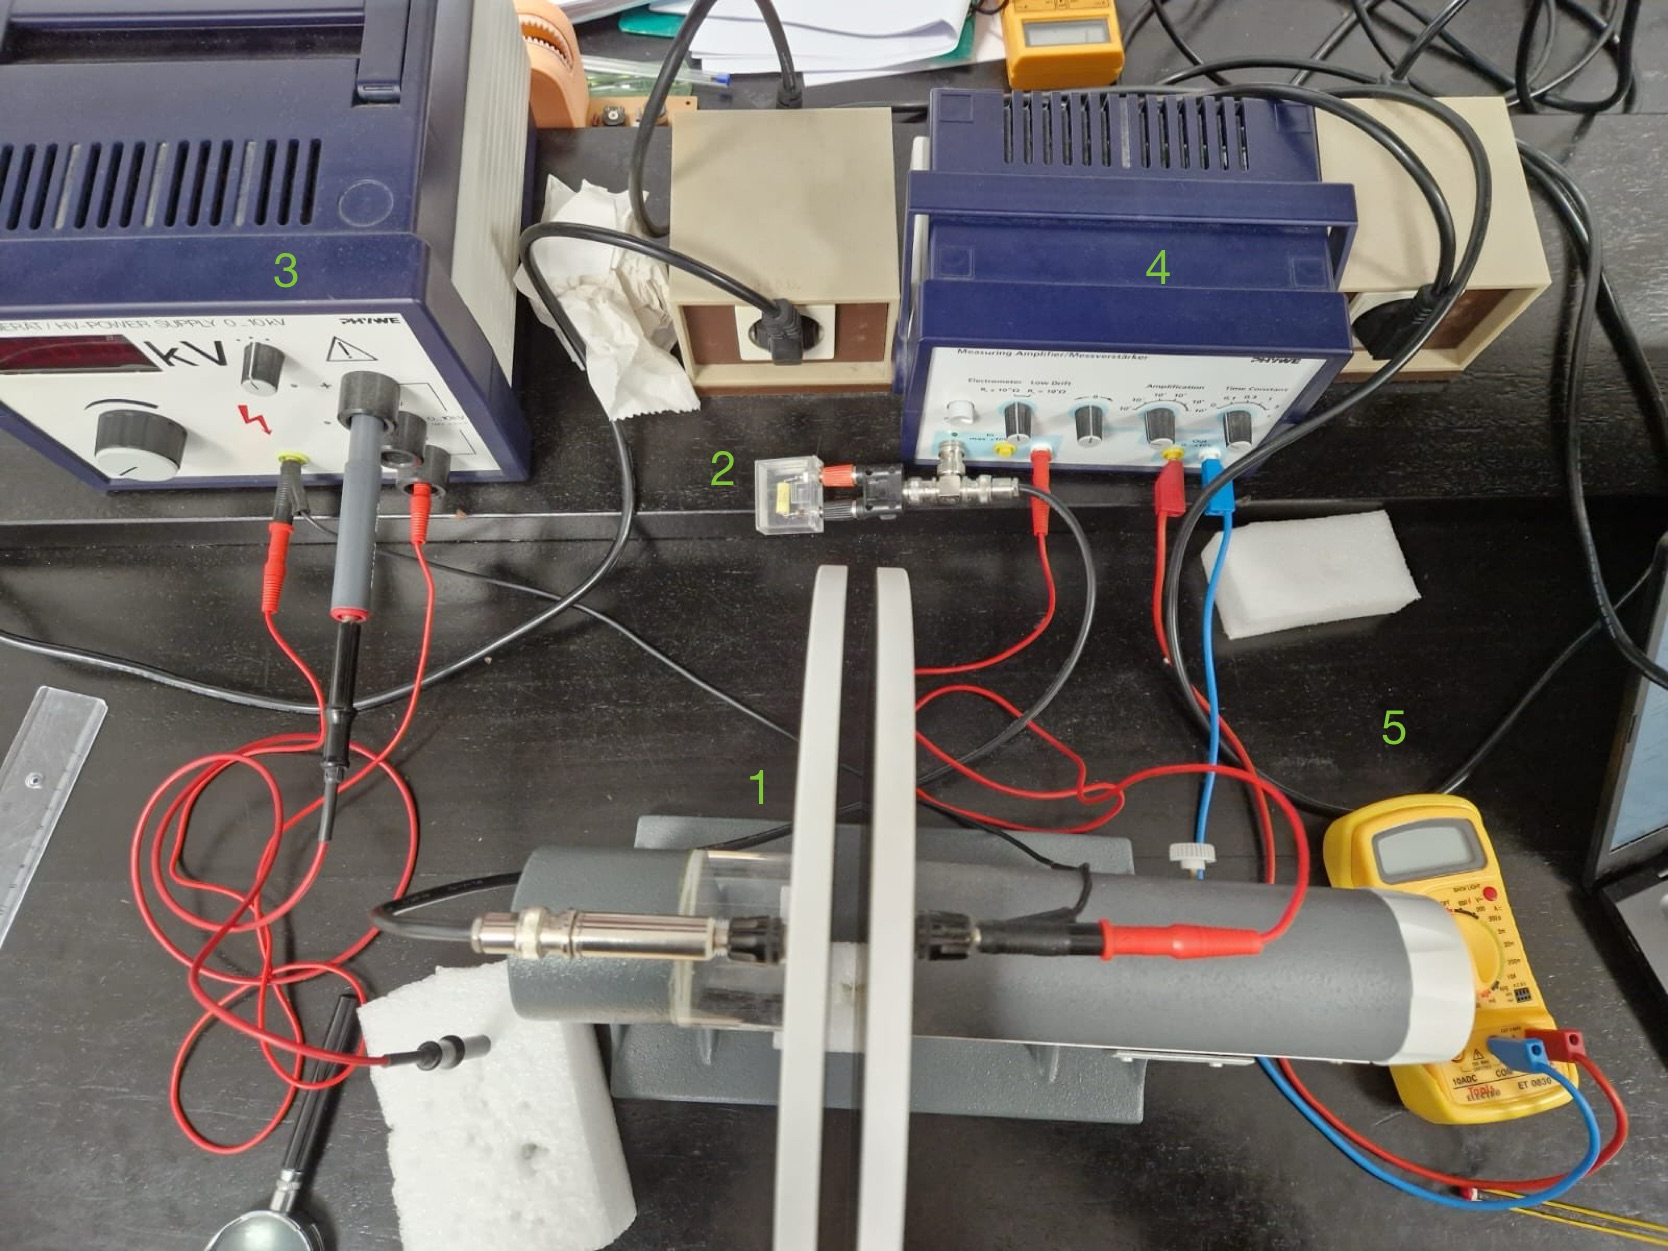
\includegraphics[width=0.75\linewidth]{materiales1.2-1.jpg}
        \subcaption{Montaje en el laboratorio}
    \end{subfigure}
    \begin{subfigure}{0.45\textwidth}
        \centering
        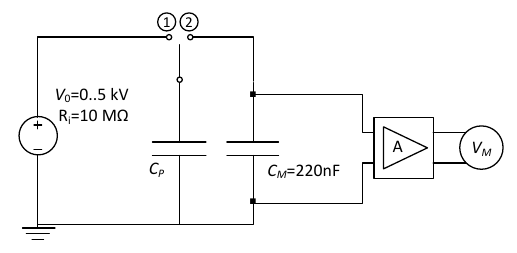
\includegraphics[width=1.15\linewidth]{montaje_esquema.png}
        \subcaption{Esquema del circuito}
    \end{subfigure}
    \caption{Montaje experimental}
    \label{Material}
\end{figure}

Esta es la configuración general, según la conexión que realicemos en 1-2 los circuitos concretos con los que trabajaremos son:

\begin{figure}[h!]
    \centering
    \begin{subfigure}{0.45\textwidth}
        \centering
        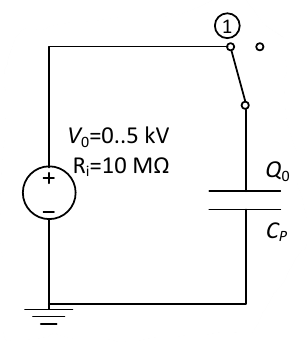
\includegraphics[width=0.65\linewidth]{conf1.png}
        \subcaption{Configuración 1, carga}
    \end{subfigure}
    \begin{subfigure}{0.45\textwidth}
        \centering
        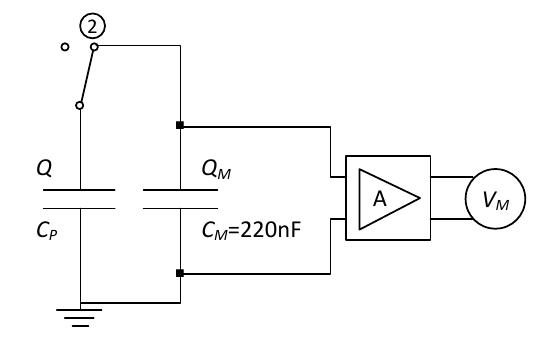
\includegraphics[width=0.95\linewidth]{conf2.png}
        \subcaption{Configuración 2, descarga}
    \end{subfigure}
    \caption{Circuitos empleados}
    \label{Material}
\end{figure}

Estas dos configuraciones representan el procedimiento experimental que vamos a llevar a cabo:

\begin{itemize}
    \item \textbf{Configuración 1}: Carga del condensador plano $C_P$ aplicándole un voltaje $V_0$, adquiriendo una carga $Q_0=C_PV_0$.
    \item \textbf{Configuración 2}: Descarga del condensador plano y carga del condensador de medida $C_M$, previamente descargado, conectándolos en paralelo. Posteriormente demostraremos que por la diferencia de órdenes de magnitud que hay entre las capacidades de los dos condensadores casi la totalidad de la carga pasará al condensador de medida, $Q_M \simeq Q_0$, por lo que midiendo el potencial del condensador de medida, $V_M$, podemos calcular la carga del condensador plano.
\end{itemize}

\newpage

El procedimiento será el siguiente:

\begin{enumerate}
    \item Empezamos con el condensador plano descargado y lo conectamos según la configuración 1 para cargarlo con $Q_0$.
    \item Desconectamos el condensador de la fuente de alimentación y lo conectamos según la configuración 2, para medir el voltaje $V_M$ con el condensador de medida.
    \item Una vez tengamos la medida de $V_M$ descargamos el condensador con el amplificador y volvemos a repetir el proceso.
\end{enumerate}

Para demostrar que el condensador plano se descarga totalmente en el condensador de medida vamos a partir del hecho de que $C_M >> C_P$ y de que están conectados en paralelo. La carga inicial es $Q_0$, por lo que las cargas que hay en los condensadores verifican $Q_0=Q_m + Q_P$. Además por estar en paralelo la diferencia de potencial en ambos condensadores es la misma, por lo que:

\begin{equation}
    V = \frac{Q_P}{C_P} = \frac{Q_M}{C_M} \Rightarrow Q_M >> Q_P
\end{equation}

Como $Q_0=Q_m + Q_P$ podemos despreciar $Q_P$ y hacer la siguiente aproximación:

\begin{equation}
    Q_0 \simeq Q_M
\end{equation}

Por último, cabe destacar que durante toda la práctica estamos cargando y descargando los condensadores, proceso que no es instantáneo ni mucho menos, sino que sigue un comportamiento exponencial. En concreto la diferencia de potencial, magnitud con la que trabajamos toda la práctica y que estamos midiendo obedece la relación:

\begin{equation}
    V(t) = V_0(1-e^{\frac{-t}{RC}})
\end{equation}

Como podemos ver en la imagen, el voltaje del condensador tiende a estabilizarse después de cierto período de tiempo. Es por eso que a la hora de realizar las medidas del voltaje del condensador de medida, $V_m$ esperamos un tiempo de carga prudencial de unos $15\;s$ en cada medida, para situarnos en el mismo punto de la curva y tomar medidas consistentes.


\begin{figure}[h!]
    \centering
    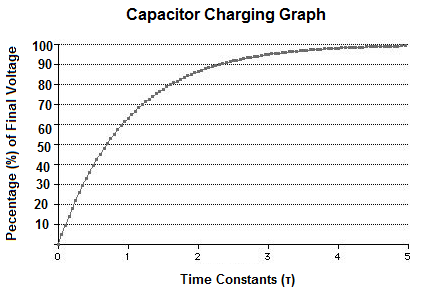
\includegraphics[width=0.45\linewidth]{curva_carga.png}
    \caption{Curva de carga, $V(t) = V_0(1-e^{\frac{-t}{RC}})$}
    \label{fig:enter-label}
\end{figure}

\newpage

Además de eso es importante destacar también que el proceso de descarga sigue una exponencial negativa del tipo:

\begin{equation}
    V=V_0 e^{\frac{-t}{RC}}
\end{equation}

Por lo que a la hora de cambiar el circuito de la configuración 1 a la 2 es importante hacerlo de forma rápida y eficaz, para minimizar la posible pérdida de carga en el proceso.

\section{Resultados experimentales y tratamiento de datos}

\subsection{Determinación de la permitividad del vacío}

En primer lugar estudiaremos la permitividad del vacío, $\epsilon_0$, para lo que trabajaremos con el condensador sin dieléctrico. Para ello emplearemos dos métodos diferentes. En primer lugar fijaremos el voltaje y variamos la distancia entre las placas para realizar un ajuste de $C_P$ frente a $1/d$. En el otro método procederemos al revés, fijaremos la distancia y variamos el voltaje para hacer un ajuste de $Q_0$ frente a $V_0$.

\subsubsection{Voltaje constante}

Para este método partimos de la relación:

\begin{equation}
    C_P = \frac{Q_0}{V_0} = \frac{\epsilon_0 S}{d}
    \label{V_cons}
\end{equation}

Donde $Q_0=C_M V_M$ como ya demostramos antes. Por tanto necesitamos medir los diferentes valores de $V_M$ para las diferentes distancias que fijamos. En la siguiente tabla podemos ver los datos obtenidos para un voltaje $V_0 =1500\pm10 \;V$:

\begin{table}[h!]
\centering
\begin{tabular}{|c|c|c|c|c|}
\hline
$d\pm 0,01\;(cm)$ & $V_M\pm0,02\;(V)$ & $Q_0\pm 4,4\;(nC)$  \\ \hline
0,20 & 2,04 & 448,8 \\ \hline 
0,22 & 1,84 & 404,8 \\ \hline 
0,24 & 1,72 & 378,4\\ \hline 
0,26 & 1,63 & 358,6 \\ \hline 
0,28 & 1,49 & 327,8 \\ \hline 
0,30 & 1,38 & 303,6 \\ \hline
\end{tabular}
\caption{Datos experimentales a voltaje fijo}
\label{tab:my-table}
\end{table}

Donde $s(Q_0)$ se obtiene trivialmente como $s(Q_0) = C_M s(V_M) = 4,4 \;nC$. A partir de estos datos podemos obtener las magnitudes necesarias para nuestra regresión lineal, que se basará en la  expresión (\ref{V_cons}):

\begin{equation}
    C_P = \frac{\epsilon_0S}{d} \sim a+ b\frac{1}{d}
\end{equation}

Donde la pendiente de la recta de regresión tiene la siguiente expresión:

\begin{equation}
    b = \epsilon_0 S \Rightarrow \epsilon_0 = \frac{b}{S} \quad s(\epsilon_0)= \frac{s(b)}{S}
\end{equation}

Los datos empleados para las regresiones fueron:

\begin{table}[h!]
\centering
\begin{tabular}{|c|c|c|c|c|c|}
\hline

$1/d\;(m^{-1})$ & $1/d\;(cm^{-1})$ & $s(1/d)\;(cm^{-1})$ & $C_P\;(F)$ & $C_P\;(pF)$ & $s(C_P)\;(pF)$ \\ \hline 
500 & 5,00 & 0,50 & $2,992\cdot 10^{-10}$ & 299,2 & 3,5\\ \hline 
455 & 4,55 & 0,41 & $2,699\cdot 10^{-10}$& 269,9 & 3,4\\ \hline 
417 & 4,17 & 0,35 & $2,523\cdot 10^{-10}$& 252,3 & 3,4\\ \hline 
385 & 3,85 & 0,30 & $2,391\cdot 10^{-10}$& 239,1 & 3,3\\ \hline 
357 & 3,57 & 0,26 & $2,185\cdot 10^{-10}$& 218,5 & 3,3\\ \hline 
333 & 3,33 & 0,22 & $2,024\cdot 10^{-10}$& 202,4 & 3,2\\ \hline

\end{tabular}
\caption{Datos empleados para las regresiones}
\label{tab:my-table}
\end{table}

\newpage

Las incertidumbres de $1/d$ y $C_P$ se obtienen por propagación de incertidumbres a partir de las expresiones:

\begin{equation}
    \begin{gathered}
        s\left(\frac{1}{d} \right) = \frac{s(d)}{d^2} \\
        s(C_P) = \sqrt{\left( \frac{s(V_0)Q_0}{V_0^2} \right)^2 + \left( \frac{s(Q_0)}{V_0} \right)^2}
    \end{gathered}
\end{equation}

En la siguiente figura podemos ver la recta de regresión obtenida:

\begin{figure}[h!]
    \centering
    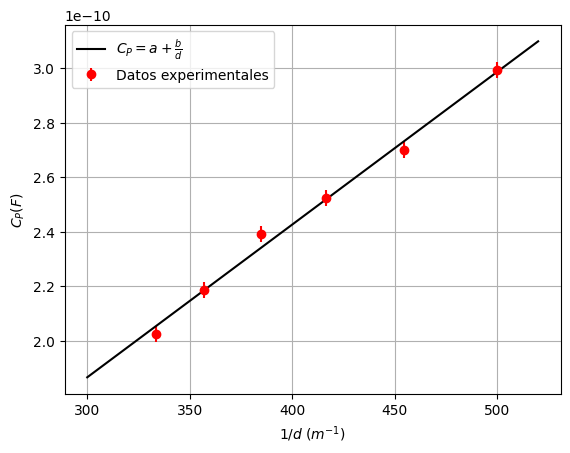
\includegraphics[width=0.65\linewidth]{v_fijo.png}
    \caption{Regresión lineal para $V_0=1,5\;kV$}
    \label{fig:enter-label}
\end{figure}

Los parámetros de la recta de regresión son los siguientes:

\begin{equation}
    a = (1,85 \pm 0,99)\cdot 10^{-11} \;F \quad \quad b = (5,60 \pm 0,24)\cdot 10^{-13} \;F\cdot m \quad \quad r = 0,996
\end{equation}

\newpage

El valor teórico de la ordenada en el origen debería ser cero, con nuestros datos de la regresión podemos afirmar que es despreciable. Una vez tenemos la pendiente de nuestra recta podemos calcular ya el valor de la constante de permitividad:

\begin{equation}
    \epsilon_0 = (1,055 \pm 0,045) \cdot 10^{-11} \;\frac{F}{m}
\end{equation}

\subsubsection{Distancia constante}

Para calcular $\epsilon_0$ a distancia constante partimos de la ecuación (\ref{V_cons}) y despejamos $Q_0$ como función lineal de $V_0$, lo que nos permite realizar una nueva regresión lineal para calcular $\epsilon_0$:

\begin{equation}
    Q_0 = \frac{\epsilon_0 S}{d} V_0 \sim a + bV_0 \Rightarrow b = \frac{\epsilon_0 S}{d}
\end{equation}

A partir de esta regresión es inmediato calcular $\epsilon_0$:

\begin{equation}
    \epsilon_0 = \frac{bd}{S} \quad s(\epsilon_0) = \sqrt{\left( \frac{b\cdot s(d)}{S}\right)^2 + \left( \frac{d\cdot s(b)}{S}\right)^2}
    \label{d_fija}
\end{equation}

Los valores de $Q_0$ se obtienen a partir de los voltajes del condensador de medida $V_M$, partiendo de la aproximación de que $Q_0 \simeq Q_M$:

\begin{equation}
    Q_0 \simeq Q_M = C_M V_M \Rightarrow s(Q_0) = C_M s(V_M)
\end{equation}

Por tanto, las medidas realizadas fueron de $V_M$ para diferentes valores de $V_0$ tomando una distancia fija $d=0,25 \pm 0,01 \;cm$. En la siguiente tabla podemos ver los datos obtenidos:

\begin{table}[h!]
\centering
\begin{tabular}{|c|c|c|c|}
\hline
$V_0\pm 10 \;(V)$ & $V_M \pm 0,02 \;(V)$ & $Q_0 \pm 0,044\cdot 10^{-7}\;(C)$ & $Q_0 \pm 4,4\;(nC)$ \\ \hline
500               & 0,86                 & $1.892 \cdot 10^{-7}$ & 189,2 \\ \hline
1000              & 1,17                 & $2.574\cdot 10^{-7}$   & 257,4 \\ \hline
1500              & 1,44                 & $3.168 \cdot 10^{-7}$   & 316,8 \\ \hline
2000              & 1,65                 & 3$.630 \cdot 10^{-7}$ & 363,0 \\ \hline
2500              & 1,80                  & $3,960 \cdot 10^{-7}$ & 396,0 \\ \hline
3000              & 2,04                 & $4.488 \cdot 10^{-7}$   & 448,8\\ \hline
\end{tabular}
\caption{Datos experimentales a distancia fija}
\label{tab:my-table}
\end{table}

Con estos datos ya podemos realizar nuestra regresión lineal, cuya recta de regresión podemos observar en la siguiente figura.

\begin{figure}[h!]
    \centering
    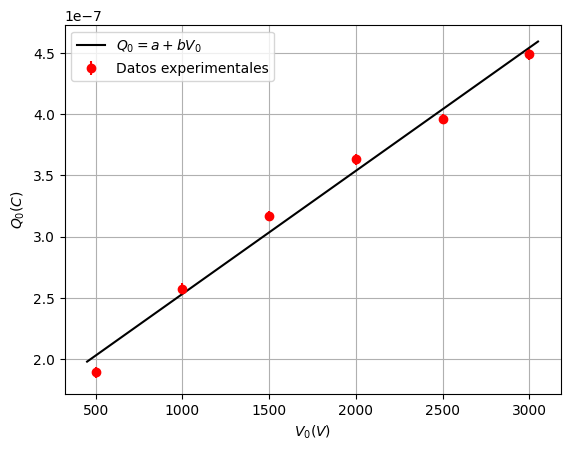
\includegraphics[width=0.65\linewidth]{d_fija.png}
    \caption{Regresión lineal para $d=0,25\;cm$}
    \label{fig:enter-label}
\end{figure}

Los parámetros de la recta de regresión son:

\begin{equation}
    a = 1,53 \pm 0,11 \cdot 10^{-8}\; C \quad b = 1,006 \pm 0,057 \cdot 10^{-10} \;F\quad r = 0,993
\end{equation}

Como en el apartado anterior, el término independiente puede ser despreciado si lo comparamos con los valores de $Q_0$ con los que trabajamos, estando un orden de magnitud por debajo. A partir de estos valores podemos calcular $\epsilon_0$ con la ecuación (\ref{d_fija}):

\begin{equation}
    \epsilon_0 = (4,74 \pm 0,33)\cdot 10^{-12} \; \frac{F}{m}
\end{equation}

\newpage

\subsection{Determinación de la permitividad de un dieléctrico}

Para la determinación de la permitividad de nuestro dieléctrico, una lámina de plástico, el procedimiento es igual que en el apartado anterior, ajustamos el dieléctrico y tomamos medidas de $V_M$ y $V_0$ con una distancia fija, en este caso $d=1,04 \pm 0,01 \;cm$. Para estudiar la permitividad relativa repetimos las medidas con la misma sustancia pero ahora sin dieléctrico. El cociente de las permitividades medidas, con y sin dieléctrico, nos permitirá obtener el valor de la permitvidad relativa de la lámina de dieléctrico según la ecuación \ref{e_r}. Las capacidades necesarias se obtienen como pendiente de la recta de regresión de $Q_0$ frente a $V_0$, donde $Q_0 = C_M V_M$.

En las siguientes tablas podemos ver las medidas tomadas con y sin el dieléctrico, a partir de las que haremos las regresiones

\begin{table}[h!]
\centering
\begin{tabular}{|c|c|c|c|}
\hline
$V_0 \pm 10\; (V)$  & $V_M \pm 0.05 \;(V)$ & $Q_0 \pm 0,11\cdot 10^{-7}\;(C)$ & $Q_0 \pm 11\;(nC)$  \\ \hline
1000 & 0,78 & $1.72\cdot 10^{-7}$ & 172\\ \hline
2000 & 1,41 & $3.10 \cdot 10^{-7}$  & 310\\ \hline
3000 & 2,51 & $5.52\cdot 10^{-7}$ & 552\\ \hline
4000 & 3,20  & $7.04 \cdot 10^{-7}$  & 704\\ \hline
5000 & 3,81 & $8.38 \cdot 10^{-7}$ & 838\\ \hline
\end{tabular}
\caption{Datos experimentales con el dieléctrico}
\label{tab:my-table}
\end{table}

\newpage

\begin{table}[h!]
\centering
\begin{tabular}{|c|c|c|c|}
\hline
$V_0 \pm 10\; (V)$  & $V_M \pm 0.05 \;(V)$ & $Q_0 \pm 0,11\cdot 10^{-7}\;(C)$ & $Q_0 \pm 11\;(nC)$  \\ \hline
1000 & 0,32 & $0,70\cdot 10^{-7}$  & 70 \\ \hline
2000 & 0,68 & $1,50\cdot 10^{-7}$ &  150\\ \hline
3000 & 0,97 & $2.13 \cdot 10^{-7}$ &  213\\ \hline
4000 & 1,26 & $2.77 \cdot 10^{-7}$ &  277\\ \hline
5000 & 1,56 & $3.43 \cdot 10^{-7}$ &  343 \\ \hline
\end{tabular}
\caption{Datos experimentales sin el dieléctrico}
\label{tab:my-table}
\end{table}

A partir de estos datos podemos hacer nuestras regresiones lineales de $Q_0$ frente a $V_0$, como en el apartado anterior. En la siguiente gráfica podemos ver las dos rectas de regresión obtenidas, lo que nos permitirá apreciar la gran diferencia que existe entre las permitividades:


\begin{figure}[h!]
    \centering
    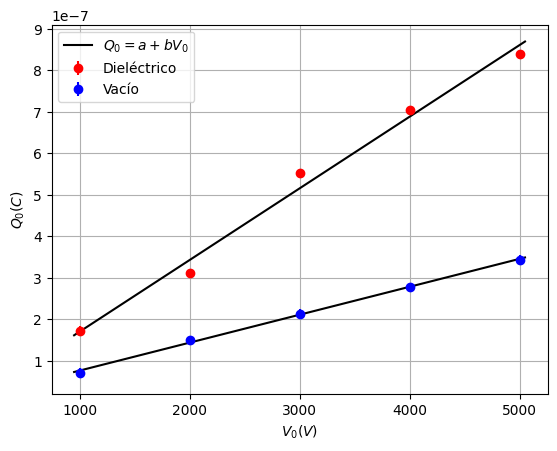
\includegraphics[width=0.65\linewidth]{dielectrico.png}
    \caption{Regresiones lineales con y sin dieléctrico}
    \label{fig:enter-label}
\end{figure}

En la siguiente tabla se especifican los parámetros obtenidos con las regresiones, la capacidad $C$ se corresponde con la pendiente de la recta de regresión, $b$:

\begin{table}[h!]
\centering
\begin{tabular}{c|c|c|}
\cline{2-3}
    & \cellcolor[HTML]{f4a9a7} Dieléctrico & \cellcolor[HTML]{c0fdfb}Vacío \\ \hline
\multicolumn{1}{|c|}{$a\pm s(a) \; (C)$} & $(-0.3 \pm 3,4)\cdot 10^{-8}$ & $(8,8 \pm 5,5) \cdot 10^{-9}$ \\ \hline
\multicolumn{1}{|c|}{$b\pm s(b) \; (F)$} & $(1,73\pm 0,10)\cdot 10^{-10}$ & $(6,73 \pm 0,17)\cdot 10^{-11}$ \\ \hline
\multicolumn{1}{|c|}{r}           & 0,994 &  0,9990 \\ \hline
\end{tabular}
\caption{Parámetros de las regresiones}
\label{tab:my-table}
\end{table}

Una vez más, como en los apartados anteriores podemos despreciar el término independiente de nuestras regresiones, pues es muy pequeño en comparación de los valores de $Q_0$ que manejamos. Una vez conocidas las capacidades del condensador, con y sin dieléctrico, podemos calcular la permitividad relativa de nuestro medio, $\epsilon_r$, con la ecuación (\ref{e_r}):

\begin{equation}
    \epsilon_r = \frac{C}{C_0} = 2,57 \pm 0,17
\end{equation}

La incertidumbre de $\epsilon_r$ se obtiene por propagación a partir de la siguiente expresión:

\begin{equation}
    s(\epsilon_r) = \sqrt{\left( \frac{s(C)}{C_0}\right)^2 + \left(\frac{s(C_0)C}{C_0^2}\right)^2}
\end{equation}

\section{Conclusiones}

Los resultados obtenidos son, en general, bastante satisfactorios. En primer lugar vamos a analizar los valores obtenidos para $\epsilon_0$, comparando el valor tabulado con los valores calculado con las regresiones lineales a voltaje y distancia constante, respectivamente, además de con la media ponderada de estos valores, que nos permitirá obtener un valor más preciso.

\begin{table}[h!]
\centering
\begin{tabular}{cc}
\textbf{Valor tabulado} $(\epsilon_0=1/\mu_0c^2)$  & $8,854187815 \cdot 10^{-12}\; F/m$ \\ 
\textbf{Voltaje constante}   & $(1,055 \pm 0,045)\cdot 10^{-11} \; F/m$ \\ 
\textbf{Distancia constante} & $(4,74 \pm 0,33)\cdot 10^{-12} \; F/m$ \\
\textbf{Media ponderada} & $(7,64 \pm 0,27)\cdot 10^{-12} \; F/m$
\end{tabular}
\caption{Comparación de los valores de $\epsilon_0$}
\label{tab:my-table}
\end{table}

Se puede ver claramente que los resultados experimentales están muy próximos del valor tabulado, estando en el mismo orden de magnitud la constante calculada a distancia constante y muy próxima la calculada a voltaje constante. Si comparamos la media ponderada de las dos regresiones con el valor tabulado podemos ver que el resultado es aún mejor, los valores están en el mismo orden de magnitud y muy próximos.

El otro gran resultado de la práctica fue calcular la permitividad relativa de nuestro dieléctrico, una lámina de plástico. La composición de la lámina es a priori desconocida pero por ser un plástico podemos tomar como referencia los polímeros orgánicos, cuya permitividad relativa a temperatura ambiente oscila entre 2 y 3 para la mayoría de compuestos. El valor obtenido es $\epsilon_r=2,57 \pm 0,17$, que se encuentra en el rango de valores esperados para un polímero orgánico, como es nuestra lámina de plástico.

Teniendo todo esto en cuenta podemos afirmar que los resultados experimentales se corresponden con los resultados que esperábamos obtener, son coherentes con la realidad. 

\section{Bibliografía}

\begin{itemize}
    \item Haynes, W. \textit{Handbook of Chemistry and Physics, 91st Edition.} (CRC Press, 2010).
    \item \textit{Capacitor charging- explained.} (s. f.). https://www.learningaboutelectronics.com/Articles\newline/Capacitor-charging.php
    \item \textit{Guiones de Prácticas}. (Departamento de electromagnetismo, 2023)
\end{itemize}

\end{document}